% В этом файле следует писать текст работы, разбивая его на
% разделы (section), подразделы (subsection) и, если нужно,
% главы (chapter).

% Предварительно следует указать необходимую информацию
% в файле SETUP.tex

%% В этот файл не предполагается вносить изменения

% В этом файле следует указать информацию о себе
% и выполняемой работе.

\documentclass [fontsize=14pt, paper=a4, pagesize, DIV=calc]%
{scrreprt}
% ВНИМАНИЕ! Для использования глав поменять
% scrartcl на scrreprt

% Здесь ничего не менять
\usepackage [T2A] {fontenc}   % Кириллица в PDF файле
\usepackage [utf8] {inputenc} % Кодировка текста: utf-8
\usepackage [russian] {babel} % Переносы, лигатуры

%%%%%%%%%%%%%%%%%%%%%%%%%%%%%%%%%%%%%%%%%%%%%%%%%%%%%%%%%%%%%%%%%%%%%%%%
% Создание макроса управления элементами, специфичными
% для вида работы (курс., бак., маг.)
% Здесь ничего не менять:
\usepackage{ifthen}
\newcounter{worktype}
\newcommand{\typeOfWork}[1]
{
	\setcounter{worktype}{#1}
}

% ВНИМАНИЕ!
% Укажите тип работы: 0 - курсовая, 1 - бак., 2 - маг.,
% 3 - бакалаврская с главами.
\typeOfWork{3}
% Считается, что курсовая и бак. бьются на разделы (section) и
% подразделы (subsection), а маг. — на главы (chapter), разделы и
%  подразделы. Если хочется,
% чтобы бак. была с главами (например, если она большая),
% надо выбрать опцию 3.

% Если при выборе 2 или 3 вы забудете поменять класс
% документа на scrreprt (см. выше, в самом начале),
% то получите ошибку:
% ./aux/appearance.tex:52: Package scrbase Error: unknown option ` chapterprefix=

%%%%%%%%%%%%%%%%%%%%%%%%%%%%%%%%%%%%%%%%%%%%%%%%%%%%%%%%%%%%%%%%%%%%%%%%
% Информация об авторе и работе для титульной страницы

\usepackage {titling}

% Имя автора в именительном падеже (для маг.)
%%\newcommand {\me}{%
%%И.\,И.~Иванов
%%}

% Имя автора в родительном падеже (для курсовой и бак.)
\newcommand {\byme}{%
A.\,A.~Мухаррам
}

% Любимый научный руководитель
\newcommand{\supervisor}%
{ст. преп. В. Н. Брагилевский}

% идентифицируем пол (только для курсовой и бак.)
\newcommand{\bystudent}{
студентки %студентки % Для курсовой: с большой буквы
}

% Год публикации
\date{2015}

% Название работы
\title{Реализация интервального времени в RabbitMQ}

% Кафедра
%
\newboolean{needchair}
\setboolean{needchair}{true} % на ФИИТ не пишется (false), на ПМИ есть (true)

\newcommand {\thechair} {%
Кафедра информатики и вычислительного эксперимента%
}

\newcommand {\direction} {%
Направление подготовки\\
Прикладная математика и информатика%
}% 

%%%%%%%%%%%%%%%%%%%%%%%%%%%%%%%%%%%%%%%%%%%%%%%%%%%%%%%%%%%%%%%%%%%%%%%%
% Другие настраиваемые элементы текста

% Листинги с исходным кодом программ: укажите язык программирования
\usepackage{listings}
\lstset{
    language=erlang,%  Язык указать здесь
    basicstyle=\small\ttfamily,
    breaklines=true,%
    showstringspaces=false%
    inputencoding=utf8x%
}
% полный список языков, поддерживаемых данным пакетом, есть,
% например, здесь (стр. 13):
% ftp://ftp.tex.ac.uk/tex-archive/macros/latex/contrib/listings/listings.pdf

% Гиперссылки: настройте внешний вид ссылок
\usepackage%
[pdftex,unicode,pdfborder=0,draft=false,%backref=page,
    hidelinks, % убрать, если хочется видеть ссылки: это
               % удобно в PDF файле, но не должно появиться на печати
    bookmarks=true,bookmarksnumbered=false,bookmarksopen=false]%
{hyperref}


\usepackage {amsmath}      % Больше математики
\usepackage {amssymb}
\usepackage {textcase}     % Преобразование к верхнему регистру
\usepackage {indentfirst}  % Красная строка первого абзаца в разделе

\usepackage {fancyvrb}     % Листинги: определяем своё окружение Verb
\DefineVerbatimEnvironment% с уменьшенным шрифтом
	{Verb}{Verbatim}
	{fontsize=\small}

% Вставка рисунков
\usepackage {graphicx}

% Общее оформление
% ----------------------------------------------------------------
% Настройка внешнего вида

%%% Шрифты

% если закомментировать всё — консервативная гарнитура Computer Modern
\usepackage{paratype} % профессиональные свободные шрифты
%\usepackage {droid}  % неплохие свободные шрифты от Google
%\usepackage{mathptmx}
%\usepackage {mmasym}
%\usepackage {psfonts}
%\usepackage{lmodern}
%var1: lh additions for bold concrete fonts
%\usepackage{lh-t2axccr}
%var2: the package below could be covered with fd-files
%\usepackage{lh-t2accr}
%\usepackage {pscyr}

% Геометрия текста

\usepackage{setspace}       % Межстрочный интервал
\onehalfspacing

\newlength\MyIndent
\setlength\MyIndent{1.25cm}
\setlength{\parindent}{\MyIndent} % Абзацный отступ
\frenchspacing            % Отключение лишних отступов после точек
\KOMAoptions{%
    DIV=calc,         % Пересчёт геометрии
    numbers=endperiod % точки после номеров разделов
}

                            % Консервативный вариант:
%\usepackage                % ручное задание геометрии
%[%                         % (не рекомендуется в проф. типографии)
%  margin = 2.5cm,
  %includefoot,
  %footskip = 1cm
%] %
%  {geometry}

%%% Заголовки



\ifthenelse{\equal{\theworktype}{2}}{%
\KOMAoptions{%
    numbers=endperiod,% точки после номеров разделов
    headings=normal,   % размеры заголовков поменьше стандартных
    chapterprefix=true,% Печатать слово Глава в магистерской
    appendixprefix=true% Печатать слово Приложение
}
}

% шрифт для оформления глав и названия содержания
\newcommand{\SuperFont}{\Large\sffamily\bfseries}

% Заголовок главы
\ifthenelse{\value{worktype} > 1}{%
\renewcommand{\SuperFont}{\Large\normalfont\sffamily}
\newcommand{\CentSuperFont}{\centering\SuperFont}
\usepackage{fncychap}
\ChNameVar{\SuperFont}
\ChNumVar{\CentSuperFont}
\ChTitleVar{\CentSuperFont}
\ChNameUpperCase
\ChTitleUpperCase
}

% Заголовок (под)раздела с абзацного отступа
\addtokomafont{sectioning}{\hspace{\MyIndent}}

\renewcommand*{\captionformat}{~---~}
\renewcommand*{\figureformat}{Рисунок~\thefigure}

%%% Оглавление
\usepackage{tocloft}

% шрифт и положение заголовка
\ifthenelse{\value{worktype} > 1}{%
\renewcommand{\cfttoctitlefont}{\hfil\SuperFont\MakeUppercase}
}{
\renewcommand{\cfttoctitlefont}{\hfil\SuperFont}
}

% слово Глава
\usepackage{calc}
\ifthenelse{\value{worktype} > 1}{%
\renewcommand{\cftchappresnum}{Глава }
\addtolength{\cftchapnumwidth}{\widthof{Глава }}
}

% Очищаем оформление названий старших элементов в оглавлении
\ifthenelse{\value{worktype} > 1}{%
\renewcommand{\cftchapfont}{}
\renewcommand{\cftchappagefont}{}
}{
\renewcommand{\cftsecfont}{}
\renewcommand{\cftsecpagefont}{}
}

\ifthenelse{\value{worktype} > 1}{%
    \renewcommand{\cftchapaftersnum}{.}
}{
\renewcommand{\cftsecaftersnum}{.}
\renewcommand{\cftsubsecaftersnum}{.}
}
%%% Списки (enumitem)

\usepackage {enumitem}      % Списки с настройкой отступов
\setlist %
{ %
  leftmargin = \parindent, itemsep=.5ex, topsep=.4ex
} %

% По ГОСТу нумерация должны быть буквами: а, б...
%\makeatletter
%    \AddEnumerateCounter{\asbuk}{\@asbuk}{м)}
%\makeatother
%\renewcommand{\labelenumi}{\asbuk{enumi})}
%\renewcommand{\labelenumii}{\arabic{enumii})}

%%% Таблицы: выбрать более подходящие

\usepackage{booktabs} % считаются наиболее профессионально выполненными
%\usepackage{ltablex}
%\newcolumntype {L} {>{---}l}

%%% Библиография

\usepackage{csquotes}        % Оформление списка литературы
\usepackage[
  backend=biber,
  hyperref=auto,
  language=auto,
  citestyle=gost-numeric,
  bibstyle=gost-numeric,
]{biblatex}
\addbibresource{biblio.bib} % Файл с лит.источниками

% Настройка величины отступа в списке
\ifthenelse{\value{worktype} < 2}{%
\defbibenvironment{bibliography}
  {\list
     {\printtext[labelnumberwidth]{%
    \printfield{prefixnumber}%
    \printfield{labelnumber}}}
     {\setlength{\labelwidth}{\labelnumberwidth}%
      \setlength{\leftmargin}{\labelwidth}%
      \setlength{\labelsep}{\dimexpr\MyIndent-\labelwidth\relax}% <----- default is \biblabelsep
      \addtolength{\leftmargin}{\labelsep}%
      \setlength{\itemsep}{\bibitemsep}%
      \setlength{\parsep}{\bibparsep}}%
      \renewcommand*{\makelabel}[1]{\hss##1}}
  {\endlist}
  {\item}
}{}

% ----------------------------------------------------------------
% Настройка переносов и разрывов страниц

\binoppenalty = 10000      % Запрет переносов строк в формулах
\relpenalty = 10000        %

\sloppy                    % Не выходить за границы бокса
%\tolerance = 400          % или более точно
\clubpenalty = 10000       % Запрет разрывов страниц после первой
\widowpenalty = 10000      % и перед предпоследней строкой абзаца

% ----------------------------


% Стили для окружений типа Определение, Теорема...
% Оформление теорем (ntheorem)

\usepackage [thmmarks, amsmath] {ntheorem}
\theorempreskipamount 0.6cm

\theoremstyle {plain} %
\theoremheaderfont {\normalfont \bfseries} %
\theorembodyfont {\slshape} %
\theoremsymbol {\ensuremath {_\Box}} %
\theoremseparator {:} %
\newtheorem {mystatement} {Утверждение} [section] %
\newtheorem {mylemma} {Лемма} [section] %
\newtheorem {mycorollary} {Следствие} [section] %

\theoremstyle {nonumberplain} %
\theoremseparator {.} %
\theoremsymbol {\ensuremath {_\diamondsuit}} %
\newtheorem {mydefinition} {Определение} %

\theoremstyle {plain} %
\theoremheaderfont {\normalfont \bfseries} 
\theorembodyfont {\normalfont} 
%\theoremsymbol {\ensuremath {_\Box}} %
\theoremseparator {.} %
\newtheorem {mytask} {Задача} [section]%
\renewcommand{\themytask}{\arabic{mytask}}

\theoremheaderfont {\scshape} %
\theorembodyfont {\upshape} %
\theoremstyle {nonumberplain} %
\theoremseparator {} %
\theoremsymbol {\rule {1ex} {1ex}} %
\newtheorem {myproof} {Доказательство} %

\theorembodyfont {\upshape} %
%\theoremindent 0.5cm
\theoremstyle {nonumberbreak} \theoremseparator {\\} %
\theoremsymbol {\ensuremath {\ast}} %
\newtheorem {myexample} {Пример} %
\newtheorem {myexamples} {Примеры} %

\theoremheaderfont {\itshape} %
\theorembodyfont {\upshape} %
\theoremstyle {nonumberplain} %
\theoremseparator {:} %
\theoremsymbol {\ensuremath {_\triangle}} %
\newtheorem {myremark} {Замечание} %
\theoremstyle {nonumberbreak} %
\newtheorem {myremarks} {Замечания} %


% Титульный лист
% Макросы настройки титульной страницы
% В этот файл не предполагается вносить изменения

%\usepackage {showframe}

% Вертикальные отступы на титульной странице
\newcommand{\vgap}{\vspace{10pt}}

% Помещение города и даты в нижний колонтитул
\usepackage{scrlayer}
\DeclareNewLayer[
  foot,
  foreground,
  contents={%
    \raisebox{\dp\strutbox}[\layerheight][0pt]{%
      \parbox[b]{\layerwidth}{\centering Ростов-на-Дону\\ \thedate%
       \\\mbox{}
       }}%
  }
]{titlepage.foot.fg}
\DeclareNewPageStyleByLayers{titlepage}{titlepage.foot.fg}


\AtBeginDocument %
{ %
  %
  \begin{titlepage}
  %
    \thispagestyle{titlepage}

    {\centering
    %
    \MakeTextUppercase {МИНИСТЕРСТВО ОБРАЗОВАНИЯ И НАУКИ РФ}

    \vgap

    Федеральное государственное автономное образовательное\\
    учреждение высшего образования\\
    \MakeTextUppercase {Южный федеральный университет}

    \vgap

  Институт математики, механики и компьютерных наук
    им.~И.\,И.~Воровича

    \vgap

    \direction

    \ifthenelse{\boolean{needchair}}{
    \vgap

    \thechair}{}

    \vspace* {\fill}

    \ifthenelse{\value{worktype} = 2}{%
    \me

    \vgap}{}

    \MakeTextUppercase{\thetitle}

    \ifthenelse{\value{worktype} = 2}{%
     \vgap

    Магистерская диссертация}{}
    \ifthenelse{\value{worktype} = 0}{
     \vgap

    Курсовая работа
    }{}%

    \vspace {\fill}

    \begin{flushright}
    \ifthenelse{\value{worktype} = 1 \OR \value{worktype} = 3}{
    Выпускная квалификационная работа\\
    на степень бакалавра%
   }{}%
    \ifthenelse{\value{worktype} = 1 \OR \value{worktype} = 0 \OR \value{worktype} = 3}{%
    \bystudent\\
    \byme
    }{}

    \vgap

    Научный руководитель:\\
    \supervisor\\
    \ifthenelse{\value{worktype} = 2}{%
    Рецензент:\\
    ученая степень, ученое звание [, должность]
    И. О. Фамилия
    }{}
  \end{flushright}

    \vspace {\fill}

  %Ростов-на-Дону

    %\thedate

  }\end{titlepage}
  %
  %
  \tableofcontents
  %
  \clearpage
} %



% Команды для использования в тексте работы


% макросы для начала введения и заключения
\newcommand{\Intro}{\addsec{Введение}}
\ifthenelse{\value{worktype} > 1}{%
    \renewcommand{\Intro}{\addchap{Введение}}%
}

\newcommand{\Conc}{\addsec{Заключение}}
\ifthenelse{\value{worktype} > 1}{%
    \renewcommand{\Conc}{\addchap{Заключение}}%
}

% Правильные значки для нестрогих неравенств и пустого множества
\renewcommand {\le} {\leqslant}
\renewcommand {\ge} {\geqslant}
\renewcommand {\emptyset} {\varnothing}

% N ажурное: натуральные числа
\newcommand {\N} {\ensuremath{\mathbb N}}

% значок С++ — используйте команду \cpp
\newcommand{\cpp}{C\nolinebreak\hspace{-.05em}%
\raisebox{.2ex}{+}\nolinebreak\hspace{-.10em}%
\raisebox{.2ex}{+}}

% Неразрывный дефис, который допускает перенос внутри слов,
% типа жёлто-синий: нужно писать жёлто"/синий.
\makeatletter
    \defineshorthand[russian]{"/}{\mbox{-}\bbl@allowhyphens}
\makeatother


\endinput

% Конец файла


\begin{document}

\Intro

Отсутствие глобального соглашения о времени может привести к возникновению ошибок в системе. В таких случаях принято говорить о необходимости синхронизации часов.
Синхронизация часов связана с пониманием порядка следования во времени событий конкурентных процессов. Она может быть полезна в тех случаях, когда необходимо синхронизировать обмен сообщениями, контролировать совместное использование ресурсов и выполнение совместной работы несколькими процессами. Таким образом, задача синхронизации в распределенной системе - обеспечить возможность принятия согласованного решения процессами о порядке следования событий. \par
Одним из вариантов решения данной проблемы является использование логических часов. Этот механизм впервые был предложен и реализован Лэсли Лампортом в 1978 году.
В своей статье ~\cite{lamport} он указал, что обычно имеет значение не точное время выполнения события процесса, а его порядок. \par
Лампорт определил логические часы как способ присвоить номер событию, где под номером понимается время, в которое наступило событие. Для каждого процесса $P_i$ определяются часы $C_i$ как функция, которая ставит в соответствие каждому событию $a$ процесса $P_i$ число  $C_i(a)$. Система в целом описывается с помощью функции $C$, которая ставит в соответствие каждому событию $b$ число $C(b)$, 
где $C(b)=$ $C_j(b)$, если $b$ - событие процесса $P_j$. С помощью этой функции можно сравнивать время наступления событий в распределенной системе.\par
Интервальные отметки времени - один из алгоритмов логических часов.  
В данной работе описан процесс разработки плагина для брокера сообщений RabbitMQ, реализующего мониторинг событий брокера на основе интервальных отметок времени. С помощью данного плагина можно восстановить цепочку событий между любыми двумя событиями системы. Под событием в RabbitMQ будет подразумеваться отправка или получение сообщения. 
\newpage

% Если typeOfWork в SETUP.tex задан как 2 или 3, то начинать
% надо не с section (раздел), а с главы (chapter)
\chapter{Логические часы}
\label{sec:examples}
Эта глава будет посвящена рассмотрению синхронизации процессов посредством нескольких алгоритмов логических часов.\par
Введем основные понятия. 
Для синхронизации логических часов Лампорт определил  не рефлексивное, транзитивное отношение под названием \textquote{происходит раньше}, которое удовлетворяет следующим 3 условиям: 
\begin{itemize}
\item Если $a$ и $b$ — события, происходящие в одном и том же процессе, и $a$
           происходит раньше, чем $b$, то отношение $a \rightarrow b$ истинно.
\item Если $a$ - отправка сообщения одним процессом, а $b$ - это получения этого сообщения другим процессом, то отношение $a \rightarrow b$ истинно.
\item Если $a \rightarrow c$ и $c \rightarrow b$, тогда из $a \rightarrow b$
\end{itemize}
Два отдельных события $a$ и $b$ конкурентные, если оба отношения $a \rightarrow b$ и $b \rightarrow a$ несправедливы. \par
Основываясь на введенном отношении и функции логических часов, запишем условие:
для любых двух событий $a$ и $b$, если $a \rightarrow b$ истинно, то $C(a) < C(b)$. Ясно, что это условие выполняется, если  события $a$ и $b$ удовлетворяют одному из условий перечисленных выше. \par
Рассмотрим последовательность событий, происходящих между тремя процессами, изображенную на рисунке 1.1.
\begin{figure}
\centering

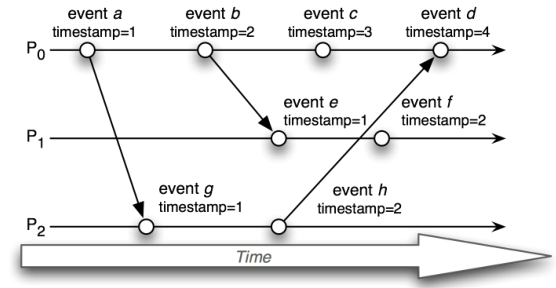
\includegraphics[width=0.5\textwidth]{img/lamport1.png}
\caption{неупорядоченная последовательность событий}
\end{figure}
Процессы запущены на разных машинах, каждая из которых имеет собственные часы и скорость работы. Каждый процесс поддерживает свой глобальный счетчик, который увеличивается на единицу перед тем, как присвоить новому событию временную отметку. Анализируя временные отметки событий, изображенных на рисунке 1.1, можно заметить несколько особенностей. Событие $g$, событие изображающее получение сообщения, посланного событием $a$, имеет такую же временную отметку, что и событие $a$, хотя совершенно ясно, что оно произошло после события $a$. Событие $e$ имеет  временную отметку меньше, чем событие отправившее ему сообщение (событие $b$).

\section{Временные отметки Лампорта}
Алгоритм Лампорта исправляет ситуацию, описанную выше, перенумеровывая временные отметки так, чтобы для событий, относящихся к отправке и получению сообщений, выполнялось отношение \textquote{происходит раньше}. \par
Правила:
\begin{itemize}
\item Каждый процесс имеет счетчик, который увеличивается на единицу  перед каждым внутренним событием процесса. Событиями процесса считается получение и отправка сообщений. 
\item К сообщению при отправке прикрепляется значение счетчика процесса.
\item При получении сообщения, если значение счетчика процесса-получателя меньше временной отметки полученного сообщения, процесс-получатель меняет значение счетчика на значение полученной временной отметки, иначе ничего не меняется. 
\end{itemize}
Применив этот алгоритм к последовательности сообщений, изображенной на рисунке 1.1, мы получим правильно упорядоченный поток сообщений среди событий, связанных 
причинно-следственной связью (рисунок 1.2). 
\begin{figure}
\centering
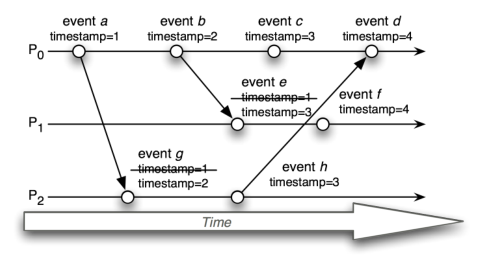
\includegraphics[width=0.5\textwidth]{img/lamport2.png}
\caption{упорядоченная последовательность событий}
\end{figure}
Каждое событие системы теперь имеет временную отметку, которая называется временной отметкой Лампорта. В условиях выполнения правил данного алгоритма, для любых двух событий системы $a$ и $b$ , если отношение $a \rightarrow b$ истинно, то $L(a) < L(b)$, где $L(x)$ - временная отметка Лампорта для события $x$. 

\section{Векторные отметки времени} 
Благодаря алгоритму Лампорта события в системе имеют единую последовательность, однако из сравнения временных отметок Лампорта $L(a)$ и $L(b)$  нельзя сделать вывод о взаимосвязи между событиями $a$ и $b$. Причинно-следственная связь может быть установлена посредством векторных
отметок времени (vector timestams)~\cite{tanenbaum}. Этот алгоритм был независимо предложен Маттерном в 1989 г.(Mattern) и Фиджем в 1991 г. (Fidge).\par
Векторная отметка времени в системе из $N$ процессов - целочисленный вектор длины $N$.\par
Правила для использования векторных отметок времени:  
\begin{itemize}
\item Каждый процесс в системе имеет свою локальную копию вектора (вектор $V_i$ для процесса $P_i$), которая инициализируется $0$: $V_i[j] = 0, i,j = 1..N$ 
\item Процесс $P_j$ перед каждым новым внутреннем событием увеличивает свою компоненту вектора на единицу: $V_j[j] = V_j[j] + 1$
\item Сообщение отправляется процессом $P_i$ вместе с векторной отметкой времени $V_i$
\item При получении сообщения процесс $P_j$ сравнивает полученную временную отметку $t$ со своим локальным вектором поэлементно, устанавливая каждую компоненту локальной временной отметки как максимум из двух значений: $V_j[i] = max(V_j[i],t[i]), i = \overline{1,N}$
\end{itemize}
Сравниваются векторные отметки по определению: 
\begin{gather*}
  V = V', \text{ если } V[i] = V'[i], i = \overline{1,N}, \\
  V \leq V',  \text{ если } V[i] \leq V'[i], i = \overline{1,N} .
\end{gather*}
С помощью алгоритма векторных часов получаем следующие утверждения.
\begin{enumerate}
\item Если отношение $a \rightarrow b$ истинно, то $V(a) < V(b)$.
\item Если $V(a) < V(b)$, то отношение $a \rightarrow b$ истинно.
\item Два события $a$ и $b$ называются конкурентными, если высказываение $V(a)\leq V(b)$ or $V(b)\leq V(a)$ ложно.
\end{enumerate}

Рассмотрим последовательность событий, изображенную на рисунке~\ref{fig:vector-algo}. Можно заметить, что события $a$ и $e$ конкурентные, так как не каждый элемент одного вектора меньше или равен соответствующему элементу другого, а события $b$ и $c$ взаимосвязаны. 

\begin{figure}
\centering
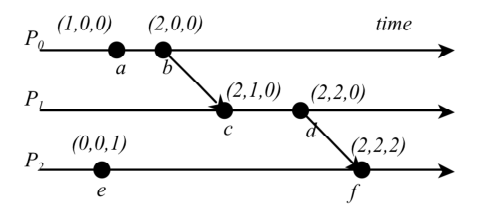
\includegraphics[width=0.5\textwidth]{img/vector.jpg}
\caption{векторный алгоритм}
\label{fig:vector-algo}
\end{figure}

\section{Счетчики дерева интервалов: Логические часы для динамических систем}
Хотя отслеживание взаимосвязей между событиями в системах с динамическим изменением числа участников возможно с помощью модифицированного алгоритма векторных часов, в большинстве таких алгоритмов наблюдается чрезмерный структурный рост, а также локализованное удаление не является поддерживаем процессов. Решение этих проблем возможно с использованием алгоритма счетчиков дерева интервалов (Interval Tree Clocks, ~\cite{itc_article}).\par
Рассмотрим, следуя ~\cite{itc_article}, возможности алгоритма интервальных отметок времени и понятия, на которых он основывается.\par
Данному механизму не требуются глобальные идентификаторы, он способен автономно создавать, удалять и повторно использовать их без помощи глобальной координации; любой объект может создать дочерний объект и количество участников может быть сокращено путем присоединения к произвольным парам объектов; метки могут расти или сокращаться, адаптируясь к динамической природе системы.\par
Механизм отслеживания причинно-следственной связи для алгоритма интервального времени моделируется посредством ряда основных операций: порождения нового процесса ($fork$), события ($event$) и слияния ($join$), воздействующих на интервальные отметки времени (логические часы), чья структура представляет собой пару (i,e), образованную идентификатором и событием, в котором и содержатся все возможные причинно-следственные связи.\par
Основная идея алгоритма заключается в том, что идентификатор каждого участника является множеством интервалов, которые используются для увеличения компоненты событие при наступлении внутреннего события процесса и для передачи последующим элементам при порождении нового процесса.\par 
Рассмотрим операции над интервальными отметками времени.\\
При выполнении операция $fork$ сохраняется компонента событие, а идентификатор делится на два непересекающихся интервала: $fork(i,e) = ((i_1,e),(i_2,e))$  
Операция $peek$ - частный случай операции $fork$: $peek(i,e)=((0,e),(i,e))$\\
Операция $event$ добавляет новое событие к временной отметке (не анонимной, $(0,e)$) так, что, если $event(i,e) = (i,e')$, то $e < e'$. 
Обнаружение причинно-следственной связи на основе интервальных отметок осуществляется посредством сравнения компонент событие.\\
Операция $join$ осуществляет слияние двух отметок: $join((i_1,e_1),(i_2,e_2)) = (i_3,e_3)$, где
$e_3 > e_2$, $e_3 > e_1$, $e_3 = e_2 \sqcup e_1$, $i_3 = f(i_2,i_3)$, $i_3$ уникален на уровне системы.
\par
Классические операции отправки, получения и синхронизации реализуются как композиция основных операций:
\begin{center}
$send = peek \circ event$\\
$receive = event \circ join$\\
$sync = fork \circ join$
\end{center}
В ITC используется исходная метка ($seed$), $(1,0)$, из которой можно получить необходимое число участников $N$ с помощью применения к ней операции $fork$ $N$ раз.
Рассмотрим пример, изображенный на рисунке 1.4. В ITC используется графическая нотация, нижний слой отметки времени - изображение идентификатора, верхние - событие. 
\begin{figure}
\centering
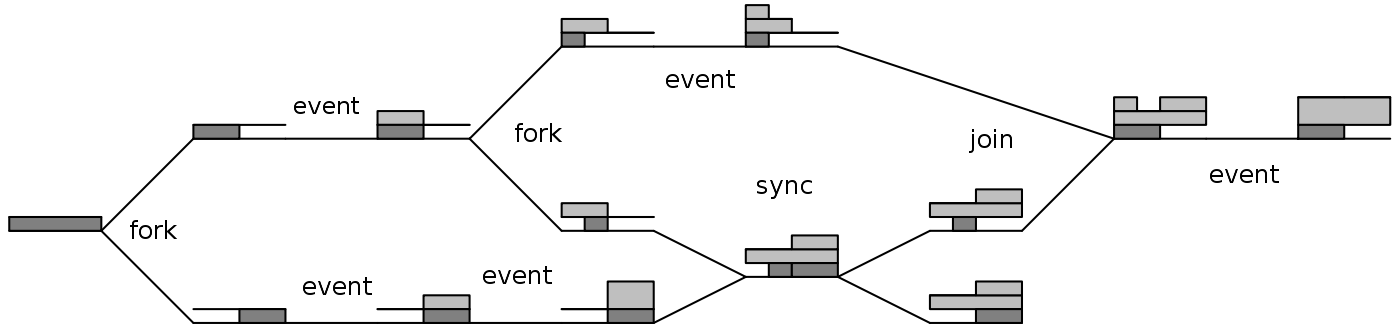
\includegraphics[width=0.8\textwidth]{img/tree.png}
\caption{интервальные отметки времени}
\end{figure}
Работа алгоритма начинается с единственного участника ($seed$) с исходной меткой, которая преобразовывается в две временные отметки под действием операции fork. На данный момент в системе два участника. В поддереве участника, соответсвующего верхней ветке дерева интервалов,происходит внутреннее событие с последующим за ним порождением нового процесса ($fork$). В поддереве участника, соответствующего нижней ветке, происходит два новых события. В этот момент число участников выросло до трех. Затем один из участников подвергается действию события, в то время как оставшиеся два участника синхронизируются. В результате с помощью операции $join$ происходит объединением двух поддеревьев. Этот пример показывает, как просто ITC адаптируется к числу участников системы.

\chapter{RabbitMQ} % написать чуть более специфицировано 
\label{sec:examples}
Мы живем в мире, в котором информация, поступающая в режиме реального времени, постоянно доступна, и написанные нами приложения нуждаются в простом, надежном, быстром способе отправки сообщений многочисленным получателям. А также часто необходимы способы изменения получателей информации, поставляемой нашими приложениями, без постоянного редактирования их кода.\par
Рассмотрим пример ~\cite{rabbitmq_in_action}. Разработчик написал аутентификационный модуль для веб-приложения \textquote{убийцы}, принадлежащего компании, в которой он работает. При каждом обращении к странице, код эффективно взаимодействует с сервером аутентификации, чтобы удостовериться в том, что пользователь действует в рамках прав доступа. Если компания потребует от программиста, написавшего модуль, организовать запись всех удавшихся и неудавшихся попыток аутентификации для дальнейшего анализа данных, то ему потребуется внести изменения в код модуля (предполагается, что с помощью аутентификационного сервера это сделать нельзя). Этого можно было бы избежать при использовании RabbitMQ.\par 
RabbitMQ - брокер сообщений с открытым кодом и сервер с организацией очередей, позволяющий приложениям обмениваться данными с помощью общего протокола или просто ставить в очередь вычисления распределенных рабочих процессов. С помощью RabbitMQ возможно связывание компонент приложения, реализованных на разных языках программирования.\par 
 Теперь представим, что программист построил решение своей задачи на основе RabbitMQ. При каждом обращении к странице, аутентификационный модуль отправляет сообщение, содержащее запрос на авторизацию, брокеру. Аутентификационный сервер подписан на очередь RabbitMQ, в которую поступают эти запросы. Как только запрос будет одобрен, сервер отправляет ответ, который RabbitMQ направляет в очередь, на которую подписан модуль. Так организуется обмен сообщениями между аутентификационным сервером и модулем. При использовании этого решения нет необходимости изменять уже написанный модуль.  Все, что теперь нужно сделать, - это написать небольшое приложение, которое связывается с брокером и подписывается на опубликованные модулем запросы.\par
В настоящее время RabbitMQ используется как небольшими стартапами , так и большими интернет-проектами. Хотя RabbitMQ берет свое начало из области финансовых конгломератов, большинством пользователей RabbitMQ теперь являются технические фирмы.\par 
\section{Передача сообщений в RabbitMQ} % здесь рассказать о протоколе немного
Рассмотрим процесс передачи сообщений в RabbitMQ, основываясь на ~\cite{rabbitmq_in_action}.\par
Передача сообщений в RabbitMQ осуществлется на основе протокола AMQP. Advanced Message Queuing Protocol (AMQP) - открытый протокол прикладного уровня для промежуточного программного обеспечения, основанное на обмене сообщениями. В 2004 году был запущен проект по созданию AMQP для финансового конгломерата JPMorgan Chase. Отличительными чертами AMQP являются ориентированность на обмен сообщениями, организация очередей, маршрутизация (точка-точка, публикация и подписка), надежность и безопасность. \par
Говоря в терминах AMQP, брокер осуществляет маршрутизацию сообщений от поставщика (producer) к подписчику (consumer). Поставщик публикует (отправляет) сообщения посредством RabbitMQ. Сообщение состоит из двух частей: данные, которые передает поставщик, и метка, с помощью которой брокер определяет, кто должен получить копию сообщения. Подписчик соединяется с брокером и подписывается на очередь. RabbitMQ отправляет поступившее в очередь сообщение одному из подписчиков. Теперь сообщение содержит только данные.\par
Перед тем как отправлять или получать сообщения необходимо установить TCP соединение между приложением и брокером и создать AMQP канал, в котором и будут происходить все действия (публикация, подписка на очередь, получение сообщения и т.д.). Канал - виртуальное соединение внутри настоящего TCP соединения, имеющее уникальный ID. Количество AMQP каналов не ограничено в пределах одного TCP соединения.\par 
Установка и разъединение TCP сессий - дорогая операция для операционной системы. Использование нескольких AMQP каналов, каждый из которых обеспечивает  для каждого потока приложения свой собственный путь к брокеру в пределах существующего TCP соединения (рис. 2.1), решение этой проблемы.\par
\begin{figure}
\centering
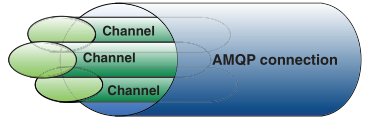
\includegraphics[width=0.5\textwidth]{img/channels.png}
\caption{каналы и соединение в AMQP}
\end{figure}
В основе AMQP маршрутизации сообщения от поставщика к подписчику (рис. 2.2) лежат три понятия: точка обмена (exchange), очередь (queue), связь (binding). Точка обмена принимает сообщения от поставщика и направляет в связанную с ней очередь в зависимости от правил, описанных в ее типе. Binding - это связь между точкой обмена и очередью. Сообщения не хранятся в точке обмена, они хранятся в очереди.\par
Подписчики получают сообщения из очереди одним из двух способов:
\begin{enumerate}
  \item С использованием AMQP команды \textit{basic.consume} пользователь подписывается на очередь и получает поступающие в нее сообщения до тех пор, пока не отпишется. 
  \item С использованием AMQP команды \textit{basic.get} пользователь отправляет запрос только на одно сообщение из очереди. 
\end{enumerate}
\begin{figure}
\centering
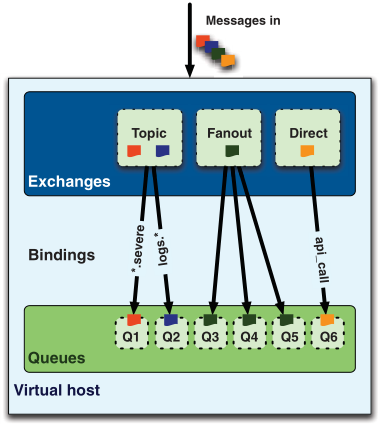
\includegraphics[width=0.4\textwidth]{img/queues.png}
\caption{AMQP стек}
\end{figure}
Если сообщение поступает в очередь без подписчиков, то оно будет там храниться до тех пор, пока не появится подписчик. В том случае, если у очереди несколько подписчиков, используется алгоритм \textquote{\textit{round-robin}}, осуществляющий циклическое распределение сообщений между подписчиками. Этот алгоритм может быть изменен с помощью опции \textit{prefetch\underline{\hspace{0.25cm}}count} метода \textit{basic\underline{\hspace{0.25cm}}qos}, в которой устанавливается максимальное количество необработанных получателем сообщений. Каждое сообщение в AMQP всегда отправляется только одному подписчику. В RabbitMQ также поддерживается механизм подтверждения сообщений. Получив сообщение, подписчик с помощью AMQP команды  \textit{basic.ack} отправляет подтверждение RabbitMQ о том, что сообщение было обработано и брокер может удалять его из очереди. Также это можно сделать, установив параметр  \textit{auto\underline{\hspace{0.25cm}}ack = true} команды \textit{basic.consume}.\par
Перейдем к рассмотрению точек обмена и их связей с очередями. Как уже было сказано ранее, поставщик публикует сообщение в точке обмена. В AMQP выбрана именно такая концепция для того, чтобы упростить маршрутизацию сообщений на основе определенных правил. Протокол предусматривает четыре типа точек обмена, каждая из которых реализует свой алгоритм маршрутизации: \textit{fanout}, \textit{direct}, \textit{topic} и \textit{headers}. Правила, из которых следует, какая очередь должна получить сообщение, называются ключами маршрутизации (\textit{routing\underline{\hspace{0.25cm}}key}). Очередь связывается с точкой обмена с помощью \textit{routing\underline{\hspace{0.25cm}}key}. Сообщение, отправленное брокеру, тоже имеет  \textit{routing\underline{\hspace{0.25cm}}key}, который будет сопоставляться с ключом маршрутизации, который изпользуется в связях точки обмена и очереди.\par
Точка обмена \textit{fanout}, как показано на рисунке 2.2, копирует все поступающие в нее сообщения во все связанные с ней очереди. Точка обмена \textit{direct} копирует сообщение в очередь, чей ключ маршрутизации равен \textit{routing\underline{\hspace{0.25cm}}key} сообщения. Брокер может определить точку обмена \textit{direct}, используя вместо имени точки обмена пустую строку, имя очереди будет использоваться как \textit{routing\underline{\hspace{0.25cm}}key}. Сообщения, отправляемые в точку обмена \textit{topic}, и связи между точкой обмена и очередью должны иметь ключ маршрутизации, состоящий из нескольких слов, разделенных точкой. Используются два специальных символа:
\begin{itemize}
\item * заменяет одно слово
\item \# заменяет любое количество слов, в том числе и нулевое
\end{itemize}
Точка обмена \textit{topic} копирует сообщение в очередь, чей ключ маршрутизации равен \textit{routing\underline{\hspace{0.25cm}}key} сообщения с учетом выше приведенных специальных символов. Точка обмена \textit{headers} осуществляет маршрутизацию, основываясь не на \textit{routing\underline{\hspace{0.25cm}}key}, а на заголовках сообщений.\par
Введем еще одно важное понятие: виртуальный хост (virtual host, vhost). В пределах каждого RabbitMQ сервера можно создать виртуальный брокер сообщений под названием vhost. Каждый виртуальный хост представляет собой RabbitMQ сервер с его собственными очередями, точками обмена, связями и правами доступа. Это полезно для разделения нескольких пользователей одного RabbitMQ сервера во избежание коллизии имен очередей и точек обмена. 
\section{Язык реализации RabbitMQ: Erlang}
RabbitMQ написан на языке Erlang с использованием  открытой телекоммуникационной платформы (OTP),
фрэймворка для создания приложений на Erlang. \par
Джо Армстронг (Joe Armstrong) начал проект по созданию Erlang для компании Ericsson в 1986 c целью улучшения разработки телекоммуникационных приложений посредством создания языка наиболее приближенного к их требованиям. В течении следующего года небольшая команда исследователей из компании Ericsson, включая Роберта Вэрдинга (Robert Virding) и Майка Уильямса (Mike Williams), помогала Армстронгу в дальнейшем развитии и усовершенствовании языка. Впоследствии в 1998 вышла бесплатная версия Erlang.\par
Erlang - функциональный язык общего назначения с сильной динамической типизацией и среда исполнения. Параллельность и передача сообщений - фундаментальные понятия для этого языка. Приложения, написанные на Erlang, часто состоят из 100 или 1000 легковесных независимых процессов, принадлежащих языку программирования, а не операционной системе, и взаимодействующих друг с другом посредством обмена сообщениями. Erlang упрощает написание распределенных приложений посредством кластера Erlang узлов, а также обеспечивает их отказоустойчивость.\par
Фрэймворк OTP - одна из отличительных черт языка программирования Erlang. OTP - множество библиотек и шаблонов проектирования для создания масштабируемых, отказоустойчивых, распределенных приложений. Одной из компонент OTP/Erlang является база данных Mnesia, являющаяся приложением, написанным на Erlang. Основная концепция OTP/Erlang - дерево наблюдения (\textit{supervision\thinspace tree}). Эта  модель организации процессов основана на идеи рабочих процессов (\textit{workers}), выполняющих вычисления, и процессов наблюдателей (\textit{supervisors}), следящих за поведением рабочих процессов. В дереве наблюдения многие процессы обладают похожей структурой. Например, процессы-наблюдатели следуют аналогичному шаблону поведения. Большинство рабочих процессов являются серверами в модели клиент-сервер, системами с конечным числом состояний  или обработчиками событий, такими как программа регистрации ошибок. Понятие поведение (\textit{behaviour}) формализует общую поведенческую модель этих процессов и схоже с понятием интерфейса в объектно-ориентированном программировании.  Основная идея заключается в разделении общей части (модуль поведения) и специфической части (функции обратного вызова). Стандартными поведениями OTP/Erlang являются \textit{gen\underline{\hspace{0.25cm}}server} (сервер в модели клиент-сервер), \textit{supervisor} (наблюдатель), \textit{gen\underline{\hspace{0.25cm}}event} (обработчик событий), \textit{gen\underline{\hspace{0.25cm}}fsm} (автомат с конечным числом состояний), \textit{application} (поведение для приложения, реализованного согласно принципам OTP). \par
\section{Архитектура RabbitMQ}
RabbitMQ реализован как приложение OTP/Erlang. Рассмотрим процесс запуска приложения RabbitMQ, основываясь на ~\cite{rabbit_boot_step}.\par Как и для любого другого приложения OTP/Erlang в каталоге с исходным кодом RabbitMQ расположен файл, реализующий поведение \textit{application}, rabbit.erl (rabbit - название приложения в данном случае). Приложение запускается при вызове функции rabbit:start/2 (rabbit - имя модуля, совпадающее с именем файла), находящейся в файле rabbit.erl.\par
Запуск RabbitMQ состоит из серии шагов, которая называется \textit{boot\thinspace steps}, отвечающей за запуск основных компонент брокера в специальном порядке. Основная идея этой концепции заключается в том, что каждая отдельная подсистема брокера определяет, от каких подсистем она зависит и работу каких подсистем делает возможной при успешном запуске. Например, нет смысла принимать запросы клиентов на соединение, если уровень, отвечающей за маршрутизацию сообщений в очередь, не активирован. Реализация этого механизма заключается в добавлении модулям erlang специальных атрибутов (деклараций),  которые определяют, как запускается шаг загрузки. Рассмотрим пример:
\begin{lstlisting}
-rabbit_boot_step({recovery,
                   [{description, "exchange, queue and binding recovery"},
                    {mfa,         {rabbit, recover, []}},
                    {requires,    empty_db_check},
                    {enables,     routing_ready}]}).
\end{lstlisting}
В данном примере приведен шаг \textit{recovery} c описанием \textquote{exchange, queue and binding recovery}. 
Перед запуском этого шага должен быть запущен шаг \textit{empty\underline{\hspace{0.25cm}}db\underline{\hspace{0.25cm}}check}, а после возможен запуск шага \textit{routing\underline{\hspace{0.25cm}}ready}. Аргумент \textit{mfa} говорит о том, что для активизации этого шага необходимо запустить функцию \textit{recover} из модуля \textit{rabbit} со списком аргументов [].\par
Шаги загрузки могут разделяться на группы. Группа шагов будет обеспечивать запуск другой группы. Например, для запуска \textit{routing\underline{\hspace{0.25cm}}ready} необходим запуск не только шага \textit{recovery}, но и многих других. Одним из этих шагов является \textit{empty\underline{\hspace{0.25cm}}db\underline{\hspace{0.25cm}}check}, который проверяет, что в Mnesia содержатся данные по умолчанию (пользователь guest, например). Некоторые шаги загрузки не требуют и не обеспечивают запуск других шагов. Они сигнализируют о том, что группа шагов завершила запуск, и следующая группа может быть запущена. Пример:
\begin{lstlisting}
{external_infrastructure,
    [{description,"external infrastructure ready"}]}
\end{lstlisting}
Опишем механизм деклараций \textit{-rabbit\underline{\hspace{0.25cm}}boot\underline{\hspace{0.25cm}}step()}. При запуске брокера создается список всех модулей, определенных в загруженных приложениях. Далее этот список сканируется на наличие атрибута \textit{rabbit\underline{\hspace{0.25cm}}boot\underline{\hspace{0.25cm}}step}. Найденные атрибуты добавляются в новый список, который обрабатывается и конвертируется в ориентированный ациклический граф, который используется для определения порядка между шагами загрузки.

\chapter{Реализация интервального времени в RabbitMQ}
RabbitMQ - система с динамическим числом участников и огромным числом событий, протекающих между поставщиками и подписчиками. В некоторых случаях для мониторинга брокера и устранения ошибок необходимо восстановить последовательность событий, протекающих в нем, и найти между ними взаимосвязь.\par
RabbitMQ предоставляет несколько средств мониторинга работы брокера. Консольная утилита \textit{rabbitmqctl} позволяет просматривать списки объектов RabbitMQ и управлять ими. Плагин \textit{rabbitmq-management} обеспечивает HTTP API для управления и мониторинга сервера RabbitMQ, как с помощью пользовательского интерфейса на основе браузера, так и с помощью  \textit{rabbitmqadmin} утилиты. Для трасировки сообщений брокера используется механизм \textit{firehose}. Но ни одно из этих средств не позволяет установить причинно-следственную связь между событиями системы. \par 
В тех случаях, когда функциональности RabbitMQ не достаточно для выполнения поставленной задачи, предусмотрен механизм расширения за счет написания плагинов. В этой главе будет описана реализация плагина для RabbitMQ с использованием алгоритма интервальных отметок времени, который будет носить название \textit{rabbitmq-itc}.

\section{Архитектура плагина}
RabbitMQ брокер - логическая группа из одного или нескольких Erlang узлов, на каждом из которых запущено приложение RabbitMQ. Все данные и объекты брокера одинаковы доступны для всех узлов кластера.\par
Плагины в RabbitMQ реализуются как приложения Erlang, следуя стандартам OTP, и запускаются на одном из узлов брокера (рис. 3.1). Для написания плагинов в RabbitMQ используется среда разработки RabbitMQ Public Umbrella.\par
\begin{figure}
\centering
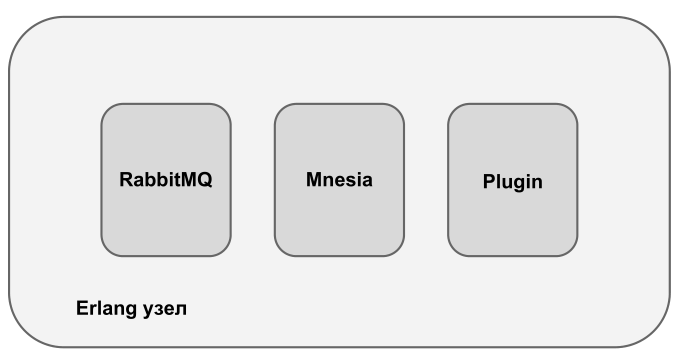
\includegraphics[width=0.55\textwidth]{img/node.png}
\caption{узлы Erlang}
\end{figure}
Плагин rabbitmq-itc состоит из 2 основных частей: серверная часть и веб-интерфейс, которые взаимодействуют посредством HTTP запросов на основе метода REST (рис. 3.2).\par
Задача сервера заключается в отслеживании событий брокера (публикация/получение сообщений) в пределах указанного с помощью веб-интерфейса  виртуального хоста и присваивании им интервальных отметок времени. Для получения всех опубликованных и доставленных подписчику сообщений используется  firehose трасировщик, который необходимо включить, указав узел и виртуальный хост, которые будут прослушиваться, перед использованием плагина (например, rabbitmqctl trace\underline{\hspace{0.25cm}}on -n rabbit@(hostname) -p <</>>). Для хранения информации о событиях брокера и их интервальных отметках плагин использует базу данных Mnesia, запущенную на том же узле брокера. Основываясь на этой информации, плагин rabbitmq-itc восстанавливает цепочку событий между двумя событиями системы c использованием реализации алгоритма интервального времени~\cite{itc}. \par
\begin{figure}
\centering
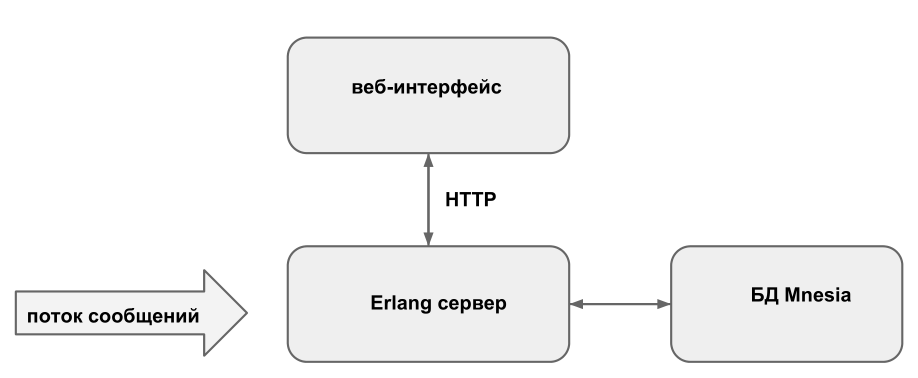
\includegraphics[width=0.7\textwidth]{img/struct.png}
\caption{архитектура плагина}
\end{figure}
\section{Запуск плагина и дерево наблюдения}
Следуя принципам OTP, информация о плагине rabbitmq-itc, его конфигурациях и других свойствах содержится в файле rabbitmq\underline{\hspace{0.25cm}}itc.app.src:
\begin{lstlisting}
{application, rabbitmq_itc,
[{description, "RabbitMQ Interval Tree Clocks"},
{vsn, "1.2.0"},
{modules, []},
{mod, {rabbitmq_itc_app,[]}},
{applications, [kernel, stdlib, rabbit, mnesia,
 rabbitmq_management]}]}.
\end{lstlisting}
\begin{figure}
\centering
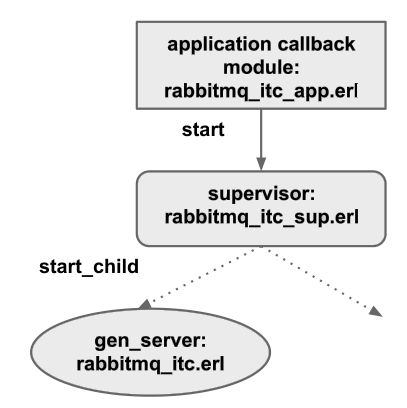
\includegraphics[width=0.45\textwidth]{img/sup.png}
\caption{дерево процессов}
\end{figure}
Структура этого файла представляет собой кортеж из 3 компонент: атом application, атом rabbitmq\underline{\hspace{0.25cm}}itc, являющийся именем плагина, и список свойств плагина, представляющих собой кортежи \{ключ,значение\}. Рассмотрим список свойств детально. Кортежи с ключами description и vsn содержат информацию о назначении и номере версии плагина соответственно. Свойство modules должно содержать список Erlang модулей, входящих в плагин. Этот список автоматически заполняется системой сборки umbrella. Свойство applications описывает список приложений, которые должны быть запущены для нормальной работы плагина. В данном случае должны быть запущены базовые приложения Erlang (\textit{kernel} и \textit{stdlib}), база данных \textit{mnesia}, приложение \textit{rabbit} и \textit{rabbitmq\underline{\hspace{0.25cm}}management} плагин, который будет использоваться для создания веб-интерфейса и организации его взаимодействия с серверной частью rabbitmq-itc. Свойство mod определяет модуль обратного вызова, реализующий поведение application, для плагина и аргументы запуска. Это означает, что при запуске плагин вызовет rabbitmq\underline{\hspace{0.25cm}}itc\underline{\hspace{0.25cm}}app:start(normal,[]). При завершении работы плагина будет вызвана функция rabbitmq\underline{\hspace{0.25cm}}itc\underline{\hspace{0.25cm}}app:stop(StartReturn), в качестве аргумента указывается значение, возвращенное при запуске плагина функцией start/2.\par 
Вызов функции start/2 из модуля rabbitmq\underline{\hspace{0.25cm}}itc\underline{\hspace{0.25cm}}app приводит к запуску процесса-наблюдателя (supervisor), поведение которого реализовано в модуле rabbitmq\underline{\hspace{0.25cm}}itc\underline{\hspace{0.25cm}}sup, с помощью функции rabbitmq\underline{\hspace{0.25cm}}itc\underline{\hspace{0.25cm}}sup:start\underline{\hspace{0.25cm}}link/0. Рассмотрим листинг модуля процесса-наблюдателя:
\begin{lstlisting}
-module(rabbitmq_itc_sup).

-behaviour(supervisor).

start_link() -> 
  supervisor:start_link({local, ?MODULE}, ?MODULE, []).

init([]) -> {ok, {{one_for_one, 3, 10},[]}}.

start_child(Args) ->
  supervisor:start_child(?MODULE,{itc, {rabbitmq_itc, start_link, [Args]},transient, ?MAX_WAIT, worker,[rabbitmq_itc]}).
\end{lstlisting}
Процесс-наблюдатель отслеживает состояние рабочих процессов и при необходимости перезапускает их. Согласно указанной в листинге кода стратегии перезапуска, если частота перезапуска в течении десяти секунд больше трёх раз, то процесс завершает работу всех дочерних процессов и завершается сам. В начале работы процесс-наблюдатель не имеет дочерних процессов, т.к. функция обратного вызова init/1 возвращает кортеж, вторая компонента которого содержит пустой список процессов. Добавление рабочего процесса (rabbitmq\underline{\hspace{0.25cm}}itc) в дерево наблюдения, изображенного на рисунке 3.3, происходит динамически при помощи функции  start\underline{\hspace{0.25cm}}child/1, которой в качестве аргумента передаётся значение виртуального хоста, при получении соответствующего HTTP запроса.\par
\section{Сервер rabbitmq\underline{\hspace{0.25cm}}itc}
Модуль rabbitmq\underline{\hspace{0.25cm}}itc - серверная часть плагина, реализующая поведение gen\underline{\hspace{0.25cm}}server. Процесс rabbitmq\underline{\hspace{0.25cm}}itc отвечает за мониторинг событий брокера и восстановление последовательностей событий на основе интервального алгоритма.\par
Перед тем как начать выполнение перечисленных выше задач, необходимо подготовить базу данных Mnesia. Для этого используется механизм rabbit\underline{\hspace{0.25cm}}boot\underline{\hspace{0.25cm}}step, описанный во второй главе. Рассмотрим шаг загрузки брокера rabbit\underline{\hspace{0.25cm}}itc\underline{\hspace{0.25cm}}mnesia:
\begin{lstlisting}
-rabbit_boot_step({rabbit_itc_mnesia,
  [{description, "rabbitmq interval tree clocks: mnesia"},
  {mfa, {?MODULE, setup_schema, []}},
  {cleanup, {?MODULE, disable_plugin, []}},
  {requires, database},
  {enables, external_infrastructure}]}).
\end{lstlisting}
На этом шаге загрузки запускается функция rabbitmq\underline{\hspace{0.25cm}}itc:setup\underline{\hspace{0.25cm}}schema/0, с помощью которой устанавливается схема базы данных для плагина: 
\begin{lstlisting}
setup_schema() ->
  mnesia:create_table(?ITC_TABLE,
  [{attributes, record_info(fields, log_record)},
  {record_name, log_record},
  {type,  ordered_set}]),
  mnesia:add_table_copy(?ITC_TABLE, node(), ram_copies),
  mnesia:wait_for_tables([?ITC_TABLE], 5000),
  ok.
\end{lstlisting}
С помощью функции mnesia:create\underline{\hspace{0.25cm}}table/2 создаётся таблица типа  ordered\underline{\hspace{0.25cm}}set, имя которой определено в макросе ?ITC\underline{\hspace{0.25cm}}TABLE. В этой таблице все записи будут иметь уникальный идентификатор. Атрибуты таблицы определены с помощью записи log\underline{\hspace{0.25cm}}record и будут введены по ходу рассмотрения реализации плагина. C помощью функций mnesia:add\underline{\hspace{0.25cm}}table\underline{\hspace{0.25cm}}copy/3 и  mnesia:wait\underline{\hspace{0.25cm}}for\underline{\hspace{0.25cm}}table/2 создается копия таблицы на узле плагина и устанавливается время ожидания доступа к таблице.\par 
При завершении работы плагина необходимо удалить таблицу ?ITC\underline{\hspace{0.25cm}}TABLE. Этот процесс описывается в свойстве  \{cleanup, \{?MODULE, disable\underline{\hspace{0.25cm}}plugin, []\}\}:
\begin{lstlisting}
disable_plugin() ->
  mnesia:delete_table(?ITC_TABLE),
  ok.
\end{lstlisting}\par
Следуя шаблону gen\underline{\hspace{0.25cm}}server, модуль rabbitmq\underline{\hspace{0.25cm}}itc разделен на две части: функции интерфейса и функции обратного вызова. Рассмотрим таблицу 3.1, описывающую взаимодействие этих функций.
\begin{table}
\centering
\caption{\label{tab:widgets} Взаимодействие функций модуля.}
\begin{tabular}{llr}
\cmidrule(r){1-2}
Функция интерфейса  & Функция обратного вызова   \\
\midrule
start\underline{\hspace{0.25cm}}link/1      & init/1   \\
all/0   & handle\underline{\hspace{0.25cm}}call/3\\
chain/1 &handle\underline{\hspace{0.25cm}}call/3\\
- & handle\underline{\hspace{0.25cm}}info/2\\
- & terminate/2\\
\bottomrule
\end{tabular}
\end{table}
Запуск процесса rabbitmq\underline{\hspace{0.25cm}}itc инициируется посредством вызова функции start\underline{\hspace{0.25cm}}link/1 процессом-наблюдателем rabbitmq\underline{\hspace{0.25cm}}itc\underline{\hspace{0.25cm}}sup. При успешной регистрации процесс rabbitmq\underline{\hspace{0.25cm}}itc вызывает функцию инициализации сервера rabbitmq\underline{\hspace{0.25cm}}itc:init/1, которая в свою очередь запускает процесс мониторинга событий брокера. Рассмотрим листинг этой функции: 
\begin{lstlisting}
init([Args]) ->
 {ok, Connection} = 
     if Args == "%2F" ->
        amqp_connection:start(#amqp_params_direct{});
                 true ->
        amqp_connection:start(#amqp_params_direct{virtual_host = list_to_binary(Args)})
     end,
 link(Connection),
 {ok, Channel} = amqp_connection:open_channel(Connection),
 link(Channel),
 #'queue.declare_ok'{queue = Q} = amqp_channel:call(Channel, #'queue.declare'{durable   = false, exclusive = true}),
 #'queue.bind_ok'{} = amqp_channel:call(Channel, #'queue.bind'{exchange = <<"amq.rabbitmq.trace">>, queue = Q,routing_key = <<"#">>}),
 #'basic.consume_ok'{} = amqp_channel:subscribe(Channel, #'basic.consume'{queue  = Q,no_ack = false}, self()),
 {ok, #state{conn = Connection, ch = Channel, queue = Q,stamp = itc:seed()}}.
\end{lstlisting}
В качестве аргумента функция init/1 получает значение виртуального хоста, устанавливает в его рамках соединение с брокером с помощью функции amqp\underline{\hspace{0.25cm}}connect:start/1 и открывает канал. С помощью функции link/1 устанавливается связь процесса rabbitmq\underline{\hspace{0.25cm}}itc с процессами Connection и Channel. Согласно механизму firehose, все опубликованные и доставленные сообщения отправляются в точку обмена типа topic <<amq.rabbitmq.trace>>. Следовательно, создав очередь и связав её с этой точкой обмена ключом маршрутизации <<\#>> с помощью AMQP команд \#'queue.declare' и \#'queue.bind' соответственно, процесс rabbitmq\underline{\hspace{0.25cm}}itc обеспечивает доставку сообщений брокера в определенную им очередь. Подписавшись на эту очередь с помощью команды amqp\underline{\hspace{0.25cm}}channel:subscribe/3, сервер начинает отслеживать события брокера. Вместе с этим начинает работу алгоритм интервального времени. Функция init/1 возвращает в качестве значения первоначальное состояние сервера, которое включает интервальную временную отметку seed (\{1,0\}).\par
В отличие от функции handle\underline{\hspace{0.25cm}}call/3 функция handle\underline{\hspace{0.25cm}}info/2 не имеет связанной с ней функции интерфейса и вызывается сервером, когда какой-нибудь связанный с ним процесс посылает ему спонтанное сообщение. Это свойство функции handle\underline{\hspace{0.25cm}}info/2 используется для получения сообщений брокера из указанной выше очереди. Рассмотрим заголов функции handle\underline{\hspace{0.25cm}}info/2:
\begin{lstlisting}
handle_info({#'basic.deliver'{}, #amqp_msg{}}, State)
\end{lstlisting}
State - состояние сервера, изменение которого происходит при появлении новых участников в системе. Вся доступная информация о событии содержится в записях \#amqp\underline{\hspace{0.25cm}}msg\{\} и \#'basic.deliver'\{\}.  С помощью записи \#'basic.deliver'\{\} можно узнать тип события и в случае, если событием является получение сообщения, очередь, в которую оно было доставлено. Запись \#amqp\underline{\hspace{0.25cm}}msg\{\} состоит из двух полей: \#'P\underline{\hspace{0.25cm}}basic'\{header = H\} и payload, содержащих заголовок сообщения и сообщение соответственно. Заголовок сообщения состоит из списка кортежей \{ключ,значение\}, благодаря которым можно узнать название точки обмена, в которой было изначально опубликовано сообщение, соединение, которое было установлено поставщиком или подписчиком в зависимости от типа события, канал, который был открыт в пределах этого соединения, и имя пользователя, к которому относится это событие. Зная эту информацию, при получении сообщения сервер применяет интервальный алгоритм.\par 
Опишем алгоритм присваивания событиям интервальных отметок времени. Под участниками в системе будут пониматься процессы пользователей, которые идентифицируются следующими свойствами: соединение с брокером (connection) и канал (channel), которые являются атрибутами таблицы ?ITC\underline{\hspace{0.25cm}}TABLE. При получении сообщения из его заголовка будет извлечена информация о соединении и канале и будет произведен поиск событий, соответствующих этим значениям, в таблице ?ITC\underline{\hspace{0.25cm}}TABLE. В случае если события не найдены, регистрируется новый участник. Для этого необходимо обратиться к состоянию сервера: \#state\{stamp = User\underline{\hspace{0.25cm}}number\} и выполнить следующую команду:
\begin{lstlisting}
{Server_stamp, User_stamp} = itc:fork(User_number)
\end{lstlisting}
Компонента событие у интервальной отметки User\underline{\hspace{0.25cm}}stamp нового участника равна нулю, а идентификатор уникален на уровне системы. Состояние сервера изменяется: \#state\{stamp = Server\underline{\hspace{0.25cm}}stamp\}. Если же уже наблюдались события участника, то обращаемся к интервальной отметке последней записи участника в таблице. Далее рассуждения будут зависеть от типа события.\par Обратимся к записи \#'basic.deliver'\{routing\underline{\hspace{0.25cm}}key = Key\}. Значение поля {routing\underline{\hspace{0.25cm}}key является бинарной строкой, первая часть которой содержит тип события. В случае, когда событием является публикация сообщения, увеличивается компонента событие интервальной отметки участника, найденной на предыдущем шаге:
\begin{lstlisting}
New_event = itc:event(User_stamp)
\end{lstlisting}
Из информации, полученной из выше указанных записей, и интервальной отметки New\underline{\hspace{0.25cm}}event формируется запись, которая помещается в таблицу ?ITC\underline{\hspace{0.25cm}}TABLE.\par
Рассмотрим схему присваивания интервальной отметки событию получения сообщения (рисунок 3.4). Согласно интервальному алгоритму операция получение является композицией операций itc:event/1 и itc:join/2 над временными отметками последнего события процесса и анонимной отметки события отправки этого сообщения. Следовательно задача состоит в том, чтобы найти в таблице информацию об отправителе сообщения ?ITC\underline{\hspace{0.25cm}}TABLE. Поиск основывается на правилах маршрутизации, которые зависят от типа точки обмена, в которой было опубликовано сообщение. Тип точки обмена определяется по названию и значению виртуального хоста с использованием функции rabbit\underline{\hspace{0.25cm}}exchange:lookup/1, определенной в RabbitMQ.
\begin{figure}
\centering
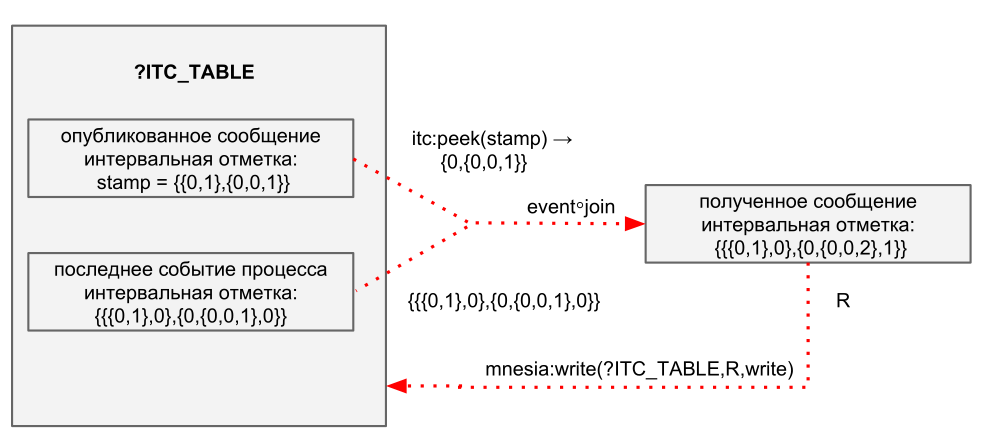
\includegraphics[width=0.8\textwidth]{img/send_recv2.png}
\caption{Процесс присваивания интервальных отметок времени}
\end{figure}
Для точки обмена типа fanout совершается поиск записи на основе существования связи с очередью, из которой подписчик получил сообщение ( rabbit\underline{\hspace{0.25cm}}binding:list\underline{\hspace{0.25cm}}for\underline{\hspace{0.25cm}}source( \#resource\{virtual\underline{\hspace{0.25cm}}host = VHost,name = Exchange, kind = exchange\})), и содержательной характеристики сообщения. Для точек обмена типа direct и topic поиск основывается как на критериях поиска для точки обмена fanout, так и на равенстве ключей маршрутизации. Когда информация об отправителе найдена, порождается интервальная отметка события подписчика, и, как показано на рисунке 3.4, сформированная запись помещается в таблицу плагина. Все транзакции проводятся с использованием функции RabbitMQ rabbit\underline{\hspace{0.25cm}}misc:execute\underline{\hspace{0.25cm}}mnesia\underline{\hspace{0.25cm}}transaction/1 для того, чтобы обеспечить непротиворечивость данных.\par
В таблице ?ITC\underline{\hspace{0.25cm}}TABLE формируется информация о событиях системы, происходивших в течение определенного времени. Сравнение интервальных отметок происходит с использованием функции itc:leq/2. Сравним две записи таблицы A и B и сделаем вывод о причинно-следственной связи между ними:
\begin{enumerate}
\item Если высказывание itc:leq(A\#log\underline{\hspace{0.25cm}}record.stamp,B\#log\underline{\hspace{0.25cm}}record.stamp) and itc:leq(B\#log\underline{\hspace{0.25cm}}record.stamp,A\#log\underline{\hspace{0.25cm}}record.stamp) истинно, то события эквивалентны.
\item Если высказывание itc:leq(A\#log\underline{\hspace{0.25cm}}record.stamp,B\#log\underline{\hspace{0.25cm}}record.stamp) or itc:leq(B\#log\underline{\hspace{0.25cm}}record.stamp,A\#log\underline{\hspace{0.25cm}}record.stamp) ложно, то события конкурентны.
\item Если высказывание not itc:leq(A\#log\underline{\hspace{0.25cm}}record.stamp,B\#log\underline{\hspace{0.25cm}}record.stamp) and itc:leq(B\#log\underline{\hspace{0.25cm}}record.stamp,A\#log\underline{\hspace{0.25cm}}record.stamp) истинно, то событие A произошло позже, чем событие B, и эти события взаимосвязаны. 
\end{enumerate}\par
Основываясь на выше перечисленных свойствах, функция handle\underline{\hspace{0.25cm}}call/3 в ответ на запрос сервера \{chain,Id\underline{\hspace{0.25cm}}1,Id\underline{\hspace{0.25cm}}2\} восстанавливает цепочку событий между событиями, соответствующими записям в таблице ?ITC\underline{\hspace{0.25cm}}TABLE с первичными ключами Id\underline{\hspace{0.25cm}}1 и Id\underline{\hspace{0.25cm}}2.
\section{Разработка веб-интерфейса}
Для удобной работы с плагином rabbitmq-itc предусмотрен веб-интерфейс  на основе архитектуры REST (рис. 3.5), с помощью которого выполняются следующие задачи:
\begin{itemize}
\item Выбор виртуального хоста, в пределах которого будет осуществляться мониторинг брокера, и запуск сервера rabbitmq\underline{\hspace{0.25cm}}itc
\item Просмотр информации о событиях брокера
\item Получение цепочки событий, восстановленной с помощью интервального алгоритма
\end{itemize}
Для доступа к интерфейсу после запуска плагина нужно перейти в браузере по ссылке  http://localhost:15672/\#/itc\underline{\hspace{0.25cm}}db и пройти аутентификацию в качестве администратора.\par
\begin{figure}
\centering
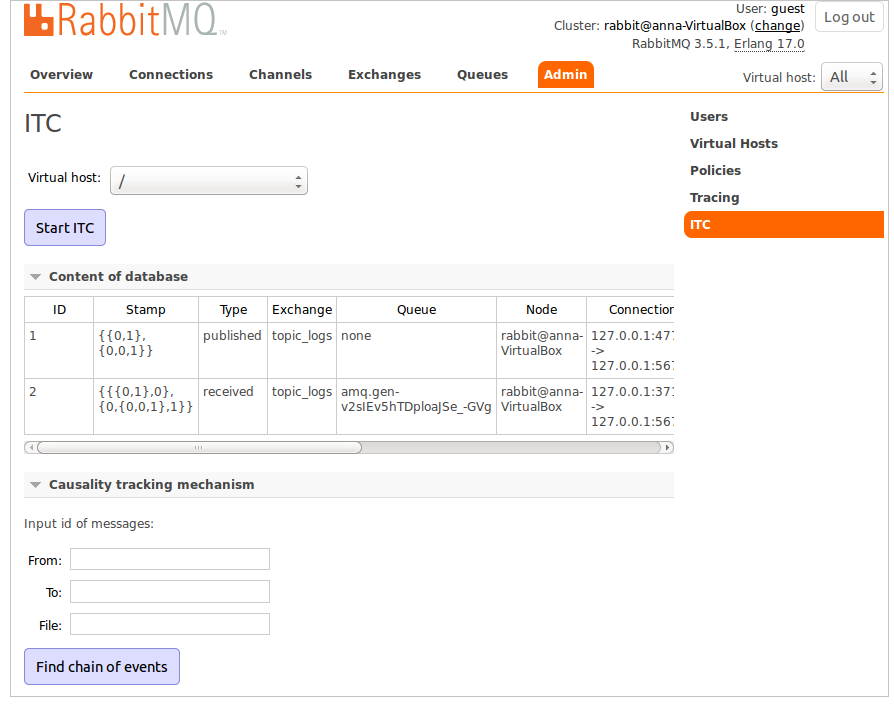
\includegraphics[width=0.8\textwidth]{img/web.png}
\caption{Веб-интерфейс}
\end{figure}
В RabbitMQ для создания REST архитектуры используется Webmachine - фрэймворк, созданный на основе веб-сервера Mochiweb. Webmachine предоставляет общий шаблон, в соответствии с которым приложения реализуют ряд функций с одинаковой сигнатурой, которые будут вызваны фрэймворком. Плагин rabbitmq-itc содержит два модуля (ресурса), соответствующих этому шаблону и обрабатывающих HTTP запросы: rabbit\underline{\hspace{0.25cm}}itc\underline{\hspace{0.25cm}}wm\underline{\hspace{0.25cm}}db и rabbit\underline{\hspace{0.25cm}}itc\underline{\hspace{0.25cm}}wm\underline{\hspace{0.25cm}}chain.\par
В плагине rabbitmq-management реализовано поведение rabbit\underline{\hspace{0.25cm}}mgmt\underline{\hspace{0.25cm}}extension. Для каждого запроса в модуле, реализующем это поведение, описывается функция какого модуля будет вызвана для обработки. Рассмотрим модуль rabbitmq\underline{\hspace{0.25cm}}itc\underline{\hspace{0.25cm}}mgmt: 
\begin{lstlisting}
-module(rabbitmq_itc_mgmt).

-behaviour(rabbit_mgmt_extension).

-export([dispatcher/0, web_ui/0]).

dispatcher() -> [{["itc_db"], rabbit_itc_wm_db, []},
                 {["itc_db",vhost,from,to,file], rabbit_itc_wm_chain, []}].

web_ui() -> [{javascript, <<"db.js">>}].
\end{lstlisting}
На запросы /itc\underline{\hspace{0.25cm}}db и /itc\underline{\hspace{0.25cm}}db/vhost/from/to/file ответ генерируется функциями модулей rabbit\underline{\hspace{0.25cm}}itc\underline{\hspace{0.25cm}}wm\underline{\hspace{0.25cm}}db и rabbit\underline{\hspace{0.25cm}}itc\underline{\hspace{0.25cm}}wm\underline{\hspace{0.25cm}}chain соответственно. Ответы формируются в формате json. В скрипте db.js определены методы для работы с REST API плагина, и страница плагина добавляется как вкладка в разделе Admin плагина rabbitmq-management. Для работы с данными в формате json используется библиотека EJS. \par
Для модуля  rabbit\underline{\hspace{0.25cm}}itc\underline{\hspace{0.25cm}}wm\underline{\hspace{0.25cm}}chain доступен метод PUT, функция этого модуля content\underline{\hspace{0.25cm}}types\underline{\hspace{0.25cm}}accepted/2 перенаправляет запросы в функцию  rabbit\underline{\hspace{0.25cm}}itc\underline{\hspace{0.25cm}}wm\underline{\hspace{0.25cm}}chain:accept\underline{\hspace{0.25cm}}content/2 :
\begin{itemize}
\item  При получении запроса вида \{vhost: <<vhost>>, from: <<undefined>>, to:<<undefined>>, file:<<undefined>>\} accept\underline{\hspace{0.25cm}}content/2 запускает дочерний процесс rabbitmq\underline{\hspace{0.25cm}}itc процесса-наблюдателя rabbitmq\underline{\hspace{0.25cm}}itc\underline{\hspace{0.25cm}}sup и передает ему значение виртуального хоста.
\item  При получении запроса вида \{vhost: <<undefined>>, from: <<id\underline{\hspace{0.25cm}}1>>, to:<<id\underline{\hspace{0.25cm}}2>>, file:<<log>>\} функция accept\underline{\hspace{0.25cm}}content/2 вызывает функцию rabbitmq\underline{\hspace{0.25cm}}itc:chain(\{id\underline{\hspace{0.25cm}}1,id\underline{\hspace{0.25cm}}2\}), которая восстанавливает цепочку событий, и полученные значения записывает в файл log.
\end{itemize}
Для модуля  rabbit\underline{\hspace{0.25cm}}itc\underline{\hspace{0.25cm}}wm\underline{\hspace{0.25cm}}db доступен метод GET, функция этого модуля content\underline{\hspace{0.25cm}}types\underline{\hspace{0.25cm}}provided/2 перенаправляет запросы в функцию  rabbit\underline{\hspace{0.25cm}}itc\underline{\hspace{0.25cm}}wm\underline{\hspace{0.25cm}}db:to\underline{\hspace{0.25cm}}json/2:\par
\begin{itemize}
\item В случае, если процесс мониторинга брокера запущен, функция json/2 вызывает функцию rabbitmq\underline{\hspace{0.25cm}}itc:all/0, которая возвращает содержимое базы данных ?ITC\underline{\hspace{0.25cm}}TABLE, и полученные значения отправляются в качестве ответа на запрос. Информация, полученная из базы данных, отображается на странице в виде таблицы (рис. 3.5).
\end{itemize}

\Conc
В рамках данной работы был разработан плагин для обнаружения причинно-следственной связи между сообщениями пользователей RabbitMQ с использованием алгоритма интервального времени. Для работы с плагином был создан интерфейс на основе REST архитектуры.\par
Использование плагина rabbitmq-itc расширяет возможности мониторнига брокера сообщений RabbitMQ. Исходный код плагина доступен в репозитории ~\cite{rabbitmq-itc}.
 


\printbibliography[heading=bibintoc
    ,title= Список литературы]


\end{document}
